\section{Setup and Notation}
\label{sec:method}

\subsection{The placeholder operator}
\label{sec:operator}

Let $\Pop \colon \Real^{n} \to \Real^{n}$ be a map, and let $\lambda \in [0,1)$
be a constant that we assume into existence.  We call the pair $(\Pop,\lambda)$
a \emph{\fixturename} whenever the following holds.

\begin{placeholderdef}
\label{def:stable}
The map $\Pop$ is \emph{placeholder-stable} with constant $\lambda$ if
$\norm{\Pop(y) - \Pop(z)} \le \lambda \norm{y - z}$ for all
$y, z \in \Real^{n}$.
\end{placeholderdef}

The iteration itself is the obvious one: starting from an arbitrary
$\iter{0} \in \Real^{n}$, set

\begin{equation}
  \label{eq:iteration}
  \iter{k+1} = \Pop\bigl(\iter{k}\bigr),
  \qquad k = 0, 1, 2, \dots
\end{equation}

Nothing in \eqref{eq:iteration} depends on the dimension $n$, which is why we
mention $n$ so often.

\begin{placeholderlem}
\label{lem:contraction}
If $(\Pop,\lambda)$ is a \fixturename{} with $\lambda < 1$, then the increments
of \eqref{eq:iteration} satisfy
$\norm{\iter{k+1} - \iter{k}} \le \lambda^{k}\norm{\iter{1} - \iter{0}}$ for
every $k \ge 0$.
\end{placeholderlem}

\begin{proof}
Apply Definition~\ref{def:stable} to consecutive iterates and unroll:
\begin{align}
  \norm{\iter{k+1} - \iter{k}}
    &\le \lambda \norm{\iter{k} - \iter{k-1}} \label{eq:step} \\
    &\le \lambda^{2} \norm{\iter{k-1} - \iter{k-2}} \nonumber \\
    &\le \lambda^{k} \norm{\iter{1} - \iter{0}} . \nonumber
\end{align}
The induction hidden in the last line is the routine one, and it is written out
in Appendix~\ref{app:details} for readers who enjoy indices.
\end{proof}

\subsection{Implementation sketch}
\label{sec:impl}

The reference implementation is four lines long and does not deserve a figure,
so we give it twice: once as code and once as a diagram.

\begin{lstlisting}[basicstyle=\ttfamily\small]
def placeholder_iteration(step, x0, tol=1e-6, max_iter=100):
    x = x0
    for k in range(max_iter):    # 100% synthetic; & no I/O here
        nxt = step(x)
        if norm(nxt - x) < tol:
            return nxt, k
        x = nxt
    return x, max_iter
\end{lstlisting}

Figure~\ref{fig:pipeline} shows the same thing with boxes.

\begin{figure}[t]
  \centering
  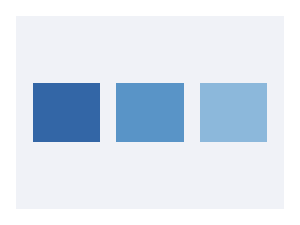
\includegraphics[width=0.55\linewidth]{figures/pipeline.pdf}
  \caption[Placeholder pipeline]{Schematic of the \fixturename: the leftmost
  block stands for whatever the reader has in mind, and the remaining blocks
  stand for it again.  About $30\%$ of the drawing is intentionally blank.}
  \label{fig:pipeline}
\end{figure}
